\subsection*{k-Nearest Neightbor}
In this problem, using the provided code, you will experiment with k-Nearest Neighbor(kNN) algorithm.

The provided kNN code performs collaborative filtering that uses other students' answers to predict whether the specific student can correctly answer some diagnostic questions. In particular, the starter code implements user-based collaborative filtering: given a user, kNN finds the closest user that similarly answered other questions and predicts the correctness based on the closest students' correctness. The core underlying assumption is that if student A has the same correct and incorrect answers on other diagnostic questions as student B, A's correctness on specific diagnostic questions matches that of student B.
\begin{itemize}
	\item [(a)] Complete a function \textbf{main} located at \textbf{knn.py} that runs KNN for different values of $k \in \{1, 6, 11, 16, 21, 26\}$ Plot and report the accuracy on the validation data as a function of k.
	\begin{center}
		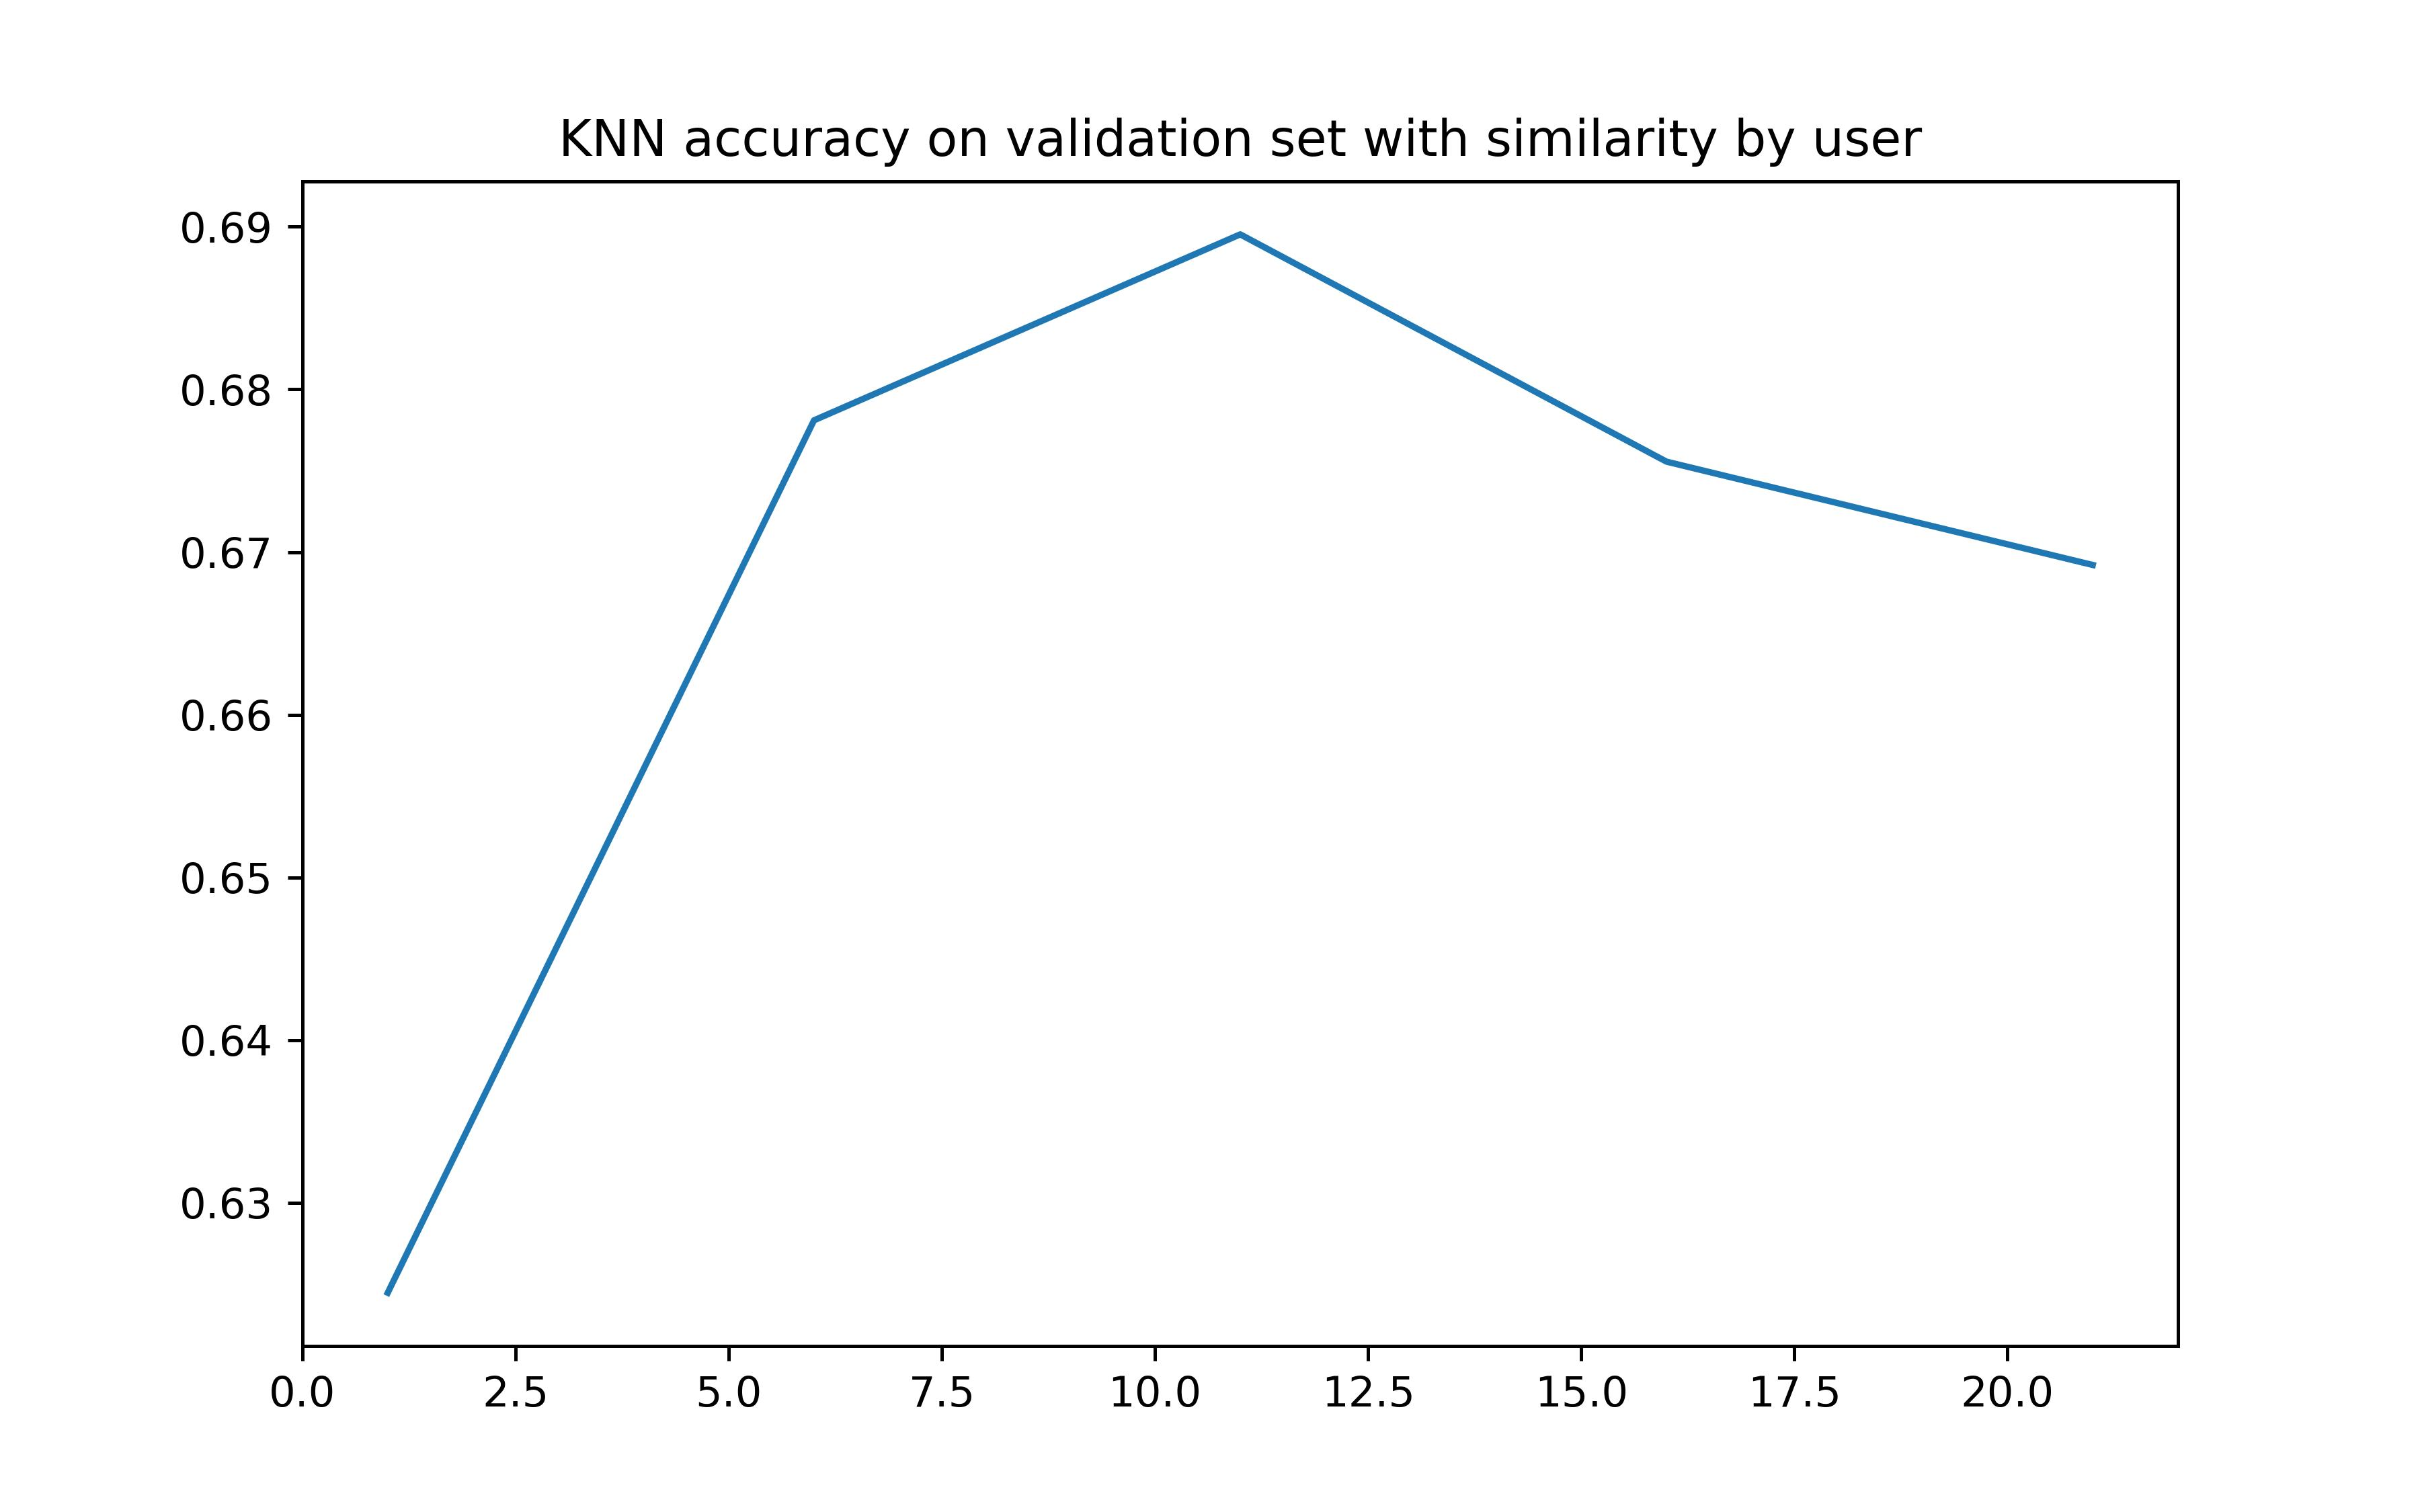
\includegraphics[scale=0.8]{../out/KNN_user.jpg}
	\end{center}
	\begin{align*}
		\text{Validation Accuracy} \mid_{k=1} &:= 0.6244707874682472\\
		\text{Validation Accuracy} \mid_{k=6} &:=0.6780976573525261 \\
		\text{Validation Accuracy} \mid_{k=11} &:= 0.6895286480383855\\
		\text{Validation Accuracy} \mid_{k=16} &:=0.6755574372001129 \\
		\text{Validation Accuracy} \mid_{k=21} &:= 0.6692068868190799\\
		\text{Validation Accuracy} \mid_{k=26} &:= 0.6522720858029918
	\end{align*}

	\item [(b)] Choose $k^*$ that has the highest performance on validation data. Report the chosen $k^*$ and the final test accuracy.
	
	Test accuracy with maximum valid accuracy with $k^* = 11$ is 0.6841659610499576
	\item[(c)] Implement a function performs item-based collaborative filtering instead of user-based collaborative filtering. Given a question, kNN finds the closest question's correctness. State the underlying assumption on item-based collaborative filtering. Repeat part (a) and (b) with item-based collaborative filtering.
	\begin{center}
		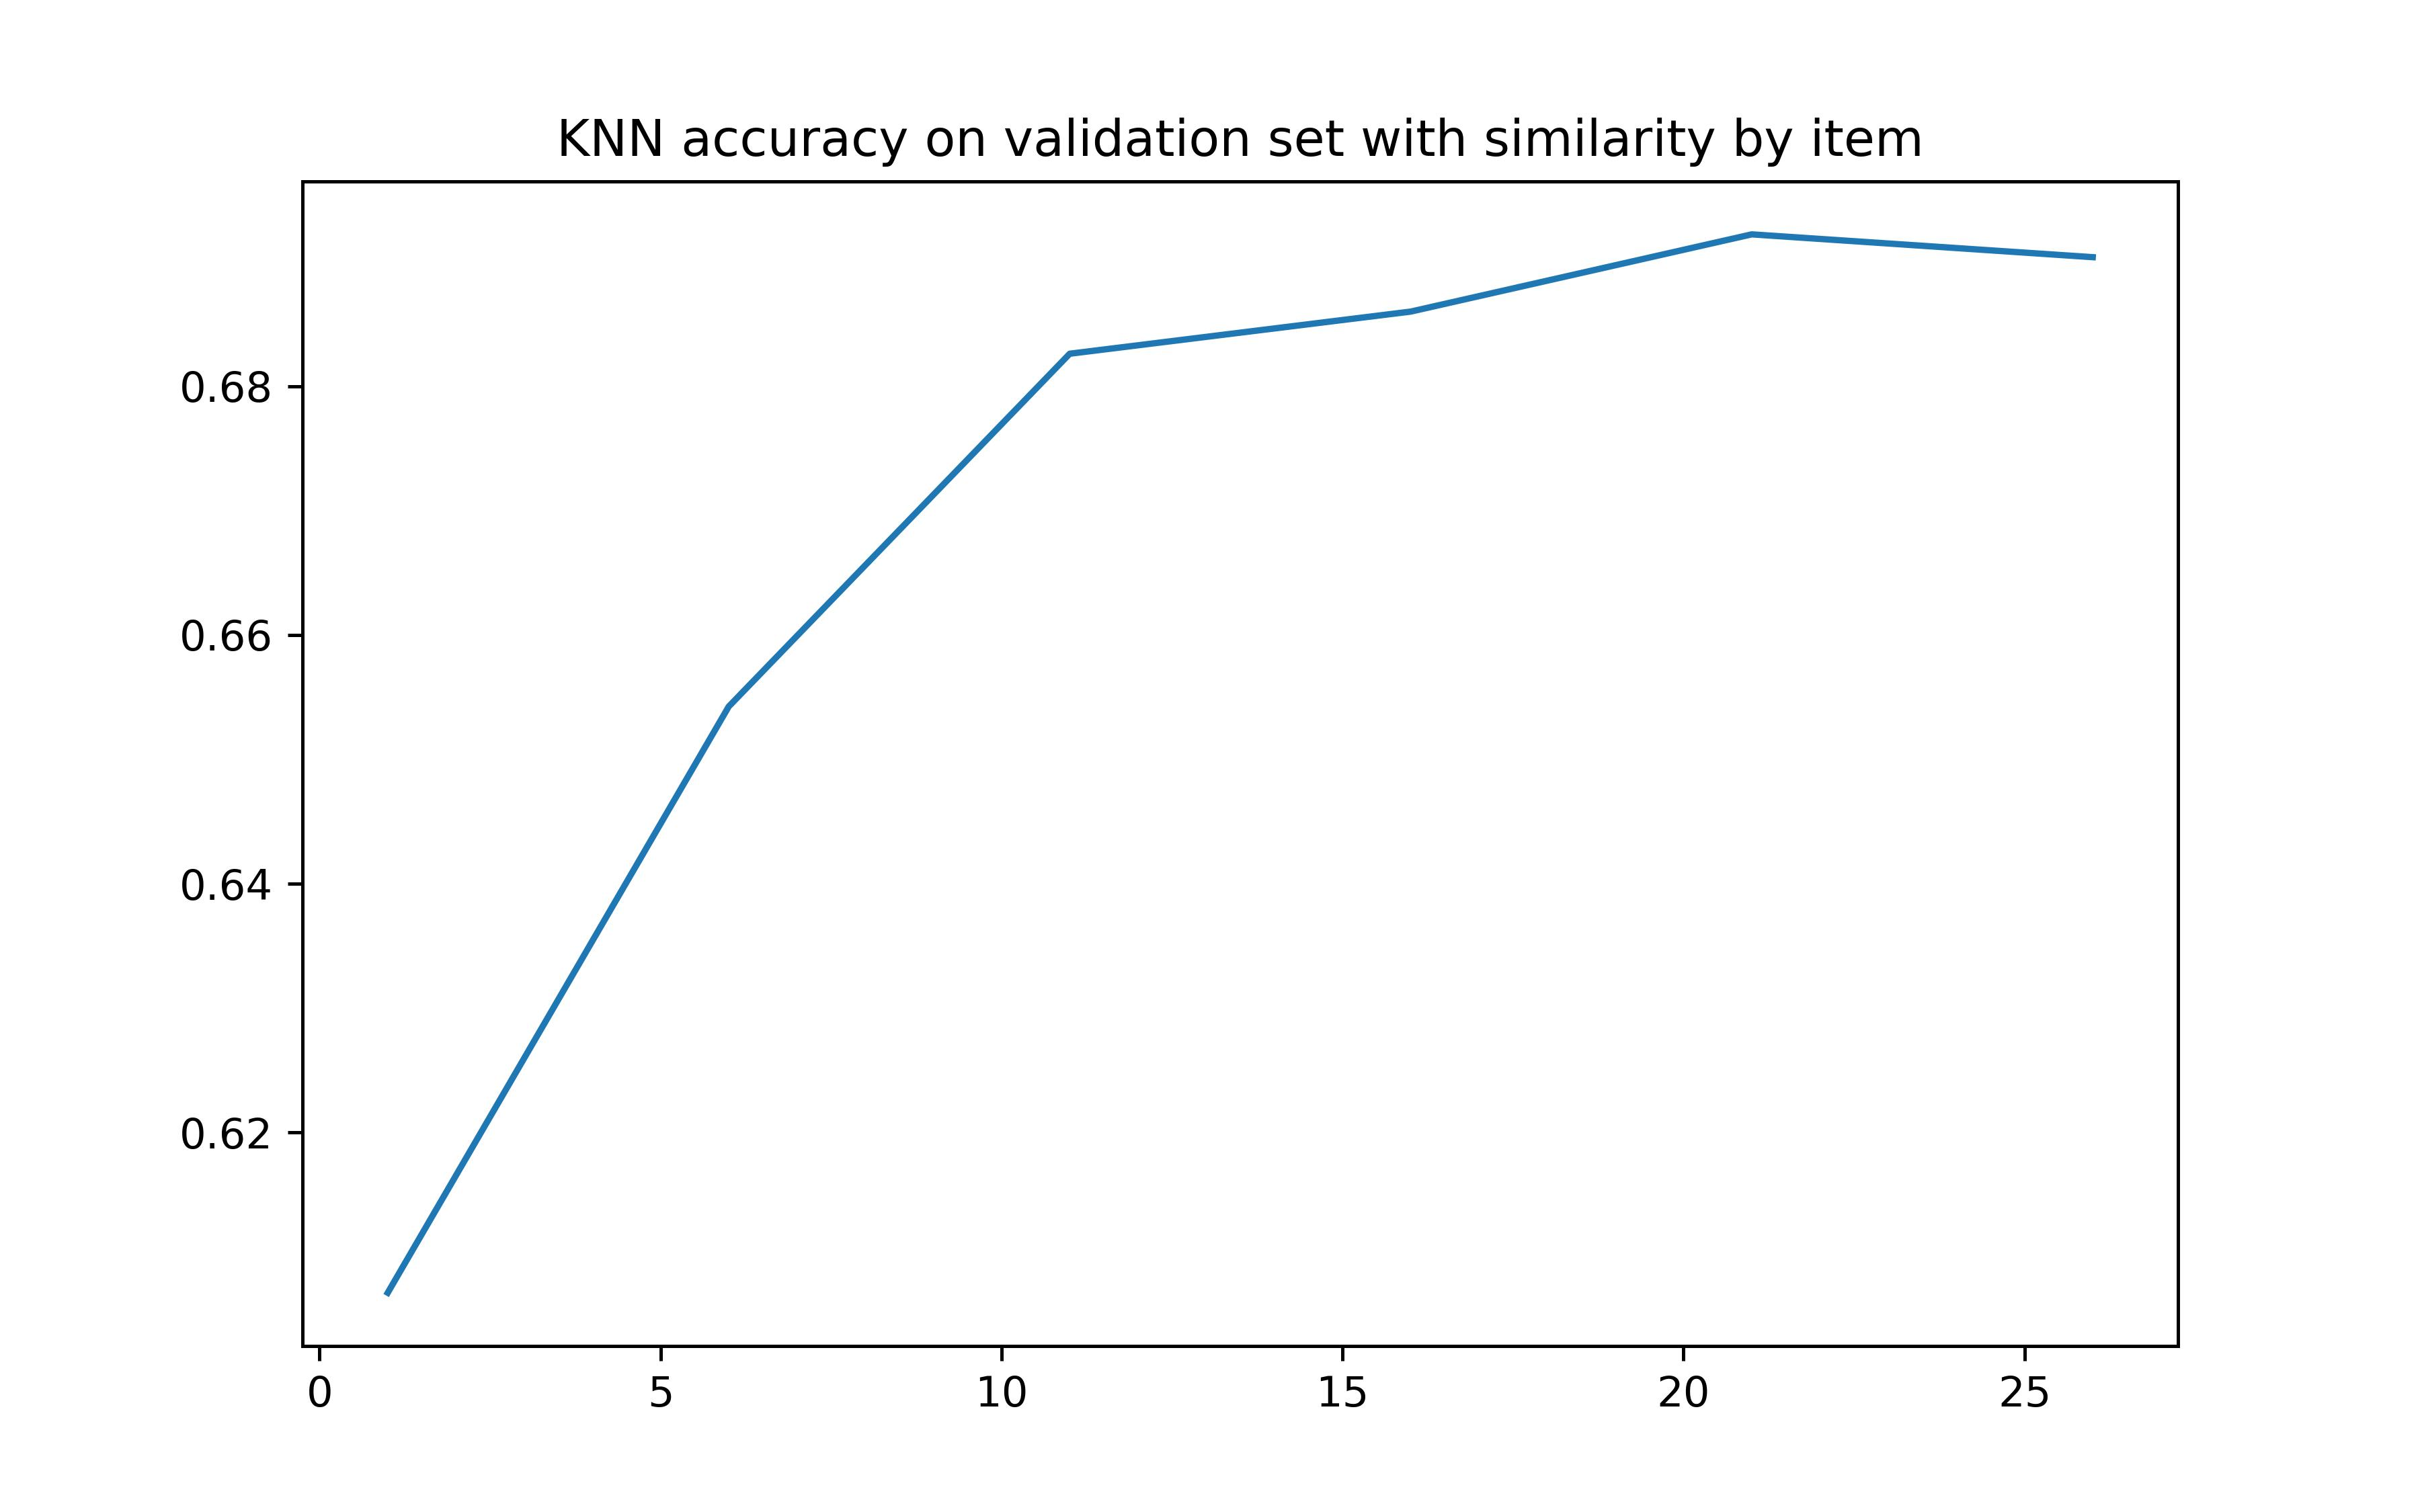
\includegraphics[scale=0.8]{../out/KNN_item.jpg}
	\end{center}
	\begin{align*}
		\text{Validation Accuracy} \mid_{k=1} &:= 0.607112616426757\\
		\text{Validation Accuracy} \mid_{k=6} &:= 0.6542478125882021\\
		\text{Validation Accuracy} \mid_{k=11} &:= 0.6826136042901496\\
		\text{Validation Accuracy} \mid_{k=16} &:= 0.6860005644933672\\
		\text{Validation Accuracy} \mid_{k=21} &:= 0.6922099915325995\\
		\text{Validation Accuracy} \mid_{k=26} &:= 0.69037538808919
	\end{align*}
	Test accuracy with maximum valid accuracy with k* = 21 is 0.6816257408975445.
	
	\item [(d)] Compare the test performance between user- and item- based collaborative filtering. State which method performs better.
	\begin{center}
		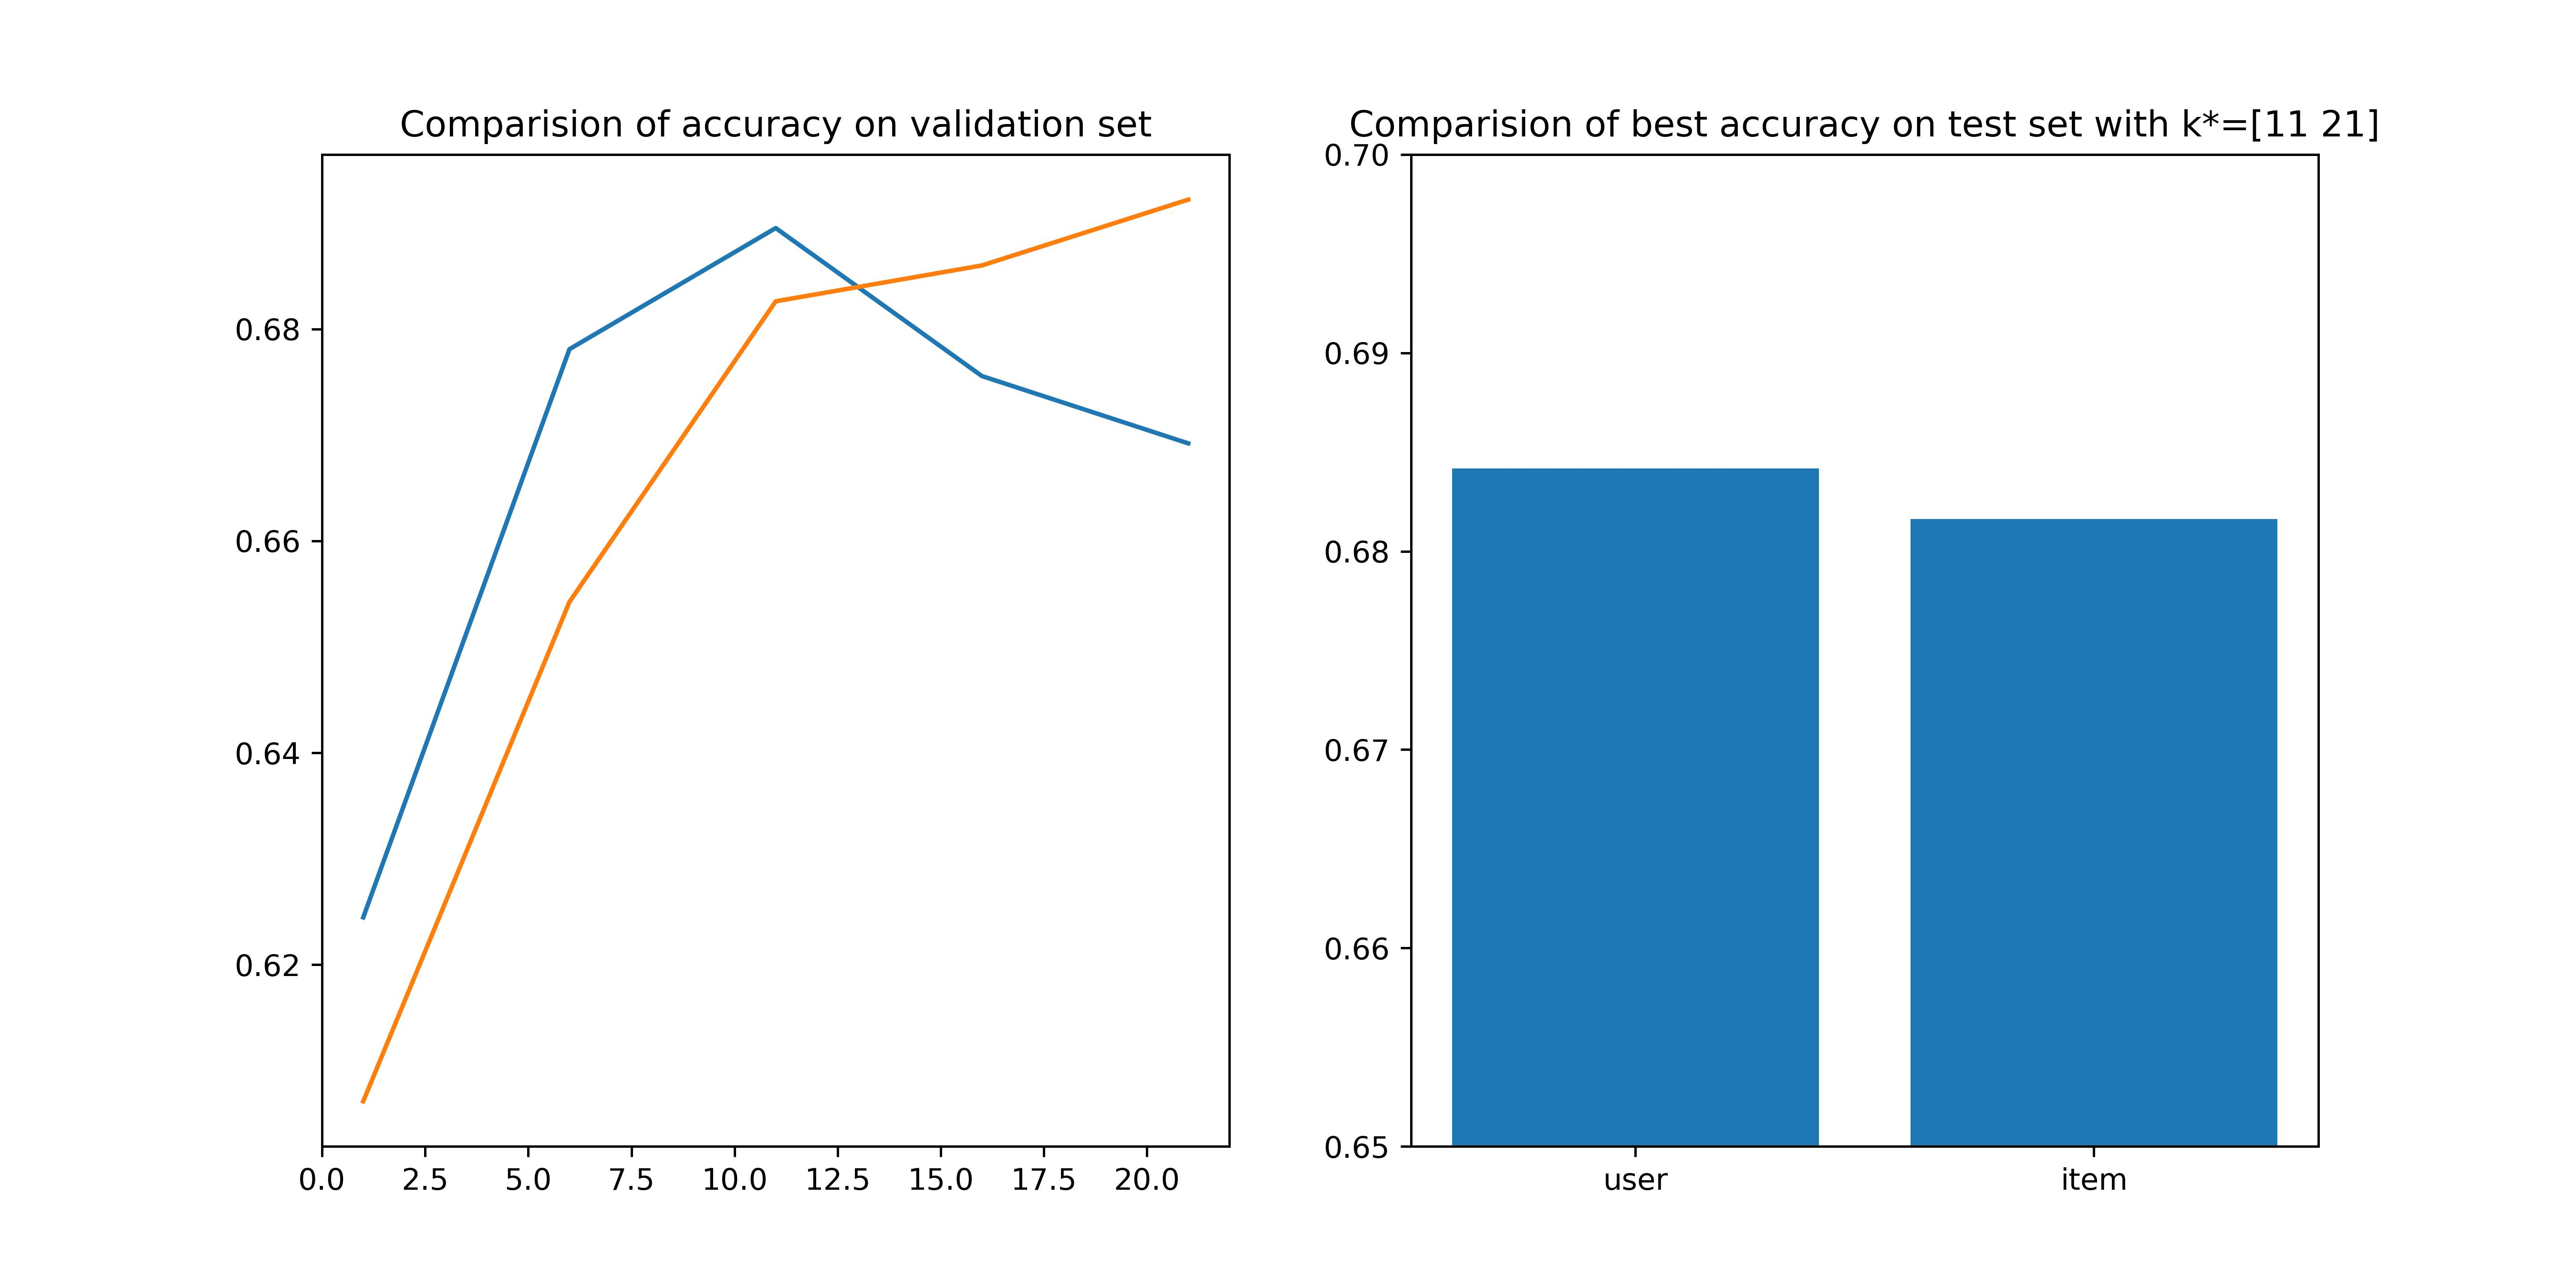
\includegraphics[scale=0.6]{../out/KNN_compare.jpg}
	\end{center}
	Based on the figure above, we claim them the user- collaborative filtering have better performance.
		\item [(e)] List at least two potential limitations of kNN for the task you are given.
		
		The curse of Dimensionality; bid computation cost on the test set.	
\end{itemize}